%%%%%%%%%%%%%%%%%%%%%%%%%%%%%%%%%%%%%%%%%%%%%%%%%%%%%%%%%%%%%%%%%%%%%%%%%%%%%%%%%%%%%%%%%%%%%%%%%%%
% Chapter 4 -> Experiments
% Author: Mingbo Cheng
%%%%%%%%%%%%%%%%%%%%%%%%%%%%%%%%%%%%%%%%%%%%%%%%%%%%%%%%%%%%%%%%%%%%%%%%%%%%%%%%%%%%%%%%%%%%%%%%%%%
\chapter{Experiments}
\label{chapter:experiments}

\graphicspath{{chapter4/figs}}



\section{Technique Validatation}
\subsection{Data}
The data we used for technique validation is two folds: (1) The data source and pre-processing of the single cell multi-modal for technical validation; (2) The simulated data for trajectory inference. We first described the data source and pre-processing for single cell multi-modal data, next we show how to simulate data for trajectory inference.

\subsubsection{multi-modal data} We make use of public multimodal data sets with two or tri-modalities in our evaluation.  The first data set is single cell cite-seq data which measures single cell RNA and surface proteins simultaneously. The human bone marrow mononuclear cells ({\texttt{BM-CITE}}) data set contains full transcriptomes and 25 surface proteins for over 30,672 cells annotated in 27 cell types~\cite{stuart2020multimodal}. This data was obtained with the ``LoadData("bmcite")'' command from package SeuratData. Next, we applied the ~\hyperref[sec:preproccessing]{pre-processing} pipeline. Another CITE-seq data used were the human peripheral blood mononuclear cells from lung ({\texttt{LUNG-CITE}}) ~\cite{buus2021improving} with 52 surface proteins. It contains 10,470 cells annotated in 22 cell types. This data was obtained from ~\url{https://tinyurl.com/253jp4sa}. The next data set contains human peripheral blood mononuclear cells ({\texttt{PBMC-multiome}}) generated by the 10x multiome technology to measure gene expression (scRNA-seq) and chromatin accessibility (scATAC-seq) on the same cells. This data contains 11,787 cells with 13 cell types annotated by 10X Genomics.  We use the scRNA-seq and scATAC-seq count matrices as provided by 10x genomics after processing with the cellranger pipeline obtained from the 
~\url{https://tinyurl.com/yw229pbf}. We also use a data set based on the SHARE-seq protocol measuring gene expression and chromatin accessibility of mouse skin cells ({\texttt{ SKIN-SHARE}})~\cite{ma2020chromatin}. This data contains 34,774 cells, which are annotated as 23 cell types. We obtain the skin scRNA-seq and scATAC-seq counts and fragments files from the Gene Expression Omnibus under accession number (\href{https://www.ncbi.nlm.nih.gov/geo/query/acc.cgi?acc=GSE140203}{GSE140203}).
%\begin{table*}
%\footnotesize
%\centering
% \caption{Major characteristics of multi-modal data sets.}
%  \label{tab:data}
%\begin{tabular}{ | l | l | l | l | l | r | r | p{0.15\linewidth} | } 
%  \hline
%  {\textbf{Dataset}} & {\textbf{Protocol}} & {\textbf{Species}}  &{\textbf{Organ}}  & {\textbf{Modalities}} &{\textbf{\#cells}}  &{\textbf{\#Cell types}}   &{\textbf{\#Features (gene/peak/protein)}} \\ 
%  \hline
%  BM-CITE  & CITE-seq & Human & Bone Marrow & RNA/protein & 30,672  & 27 & 17,009/-/25 \\
%  \hline
%  LUNG-CITE  & CITE-seq & Human & PBMC\&Lung & RNA/protein & 10,470  & 22 & 33,514/-/52 \\
%  \hline
%  PBMC-Multiome  & Multiome & Human  & PBMC & RNA/ATAC & 11,787 & 13 & 36,610/108,377/- \\ 
%  \hline
%  Skin-SHARE  & SHARE-seq & Mouse & Skin & RNA/ATAC & 34,774 & 23 & 23,296/344,592/- \\ 
%  \hline
%  PBMC-TEA  & TEA-seq  & Human & PBMC & RNA/ATAC/epitope & 25,517 & 12 &  36,601/128,853/47\\ 
%  \hline
%  PBMC-DOGMA  & DOGMA-seq & Human & PBMC & RNA/ATAC/protein & 13,763  & 27 & 36,495/68,963/210 \\
%  \hline
%\end{tabular}
%\end{table*}




\begin{table}[!ht]
	\footnotesize
	\centering
	\begin{tabular}{lllllrrp{0.15\linewidth}}
		\toprule
		{\textbf{Dataset}} & {\textbf{Protocol}} & {\textbf{Species}}  &{\textbf{Organ}}  & {\textbf{Modalities}} &{\textbf{\#cells}}  &{\textbf{\#Cell types}}   &{\textbf{\#Features (gene/peak/protein)}} \\ 
		\midrule
		  BM-CITE  & CITE-seq & Human & Bone Marrow & RNA/protein & 30,672  & 27 & 17,009/-/25 \\
		  LUNG-CITE  & CITE-seq & Human & PBMC\&Lung & RNA/protein & 10,470  & 22 & 33,514/-/52 \\
		  PBMC-Multiome  & Multiome & Human  & PBMC & RNA/ATAC & 11,787 & 13 & 36,610/108,377/- \\ 
		  Skin-SHARE  & SHARE-seq & Mouse & Skin & RNA/ATAC & 34,774 & 23 & 23,296/344,592/- \\ 
		  PBMC-TEA  & TEA-seq  & Human & PBMC & RNA/ATAC/epitope & 25,517 & 12 &  36,601/128,853/47\\ 
		  PBMC-DOGMA  & DOGMA-seq & Human & PBMC & RNA/ATAC/protein & 13,763  & 27 & 36,495/68,963/210 \\
		\bottomrule
	\end{tabular}
	\vspace{0.1cm}
	\caption[Major characteristics of multi-modal data sets]{Major characteristics of multi-modal data sets.}
	\label{tab:MOJITOO_DATA}
\end{table}


A tri-modal data set of human PBMCs is measured with the DOGMA-seq protocol~\cite{mimitou2021scalable}. This provides RNA, ATAC and epitope sequencing of the same cells ({\texttt{PBMC-DOGMA}}). We use data under low-loss lysis conditions, which contains 13,763 cells in 27 cell types. We download count matrices as provided by the authors ~\url{https://osf.io/6kr4v/}. A second tri-modal dataset is based on human PBMCs measured with the TEA-seq protocol~\cite{swanson2021simultaneous}. It contains transcripts, epitopes and chromatin accessibility of 25,517 PBMCs grouped into 12 cell types ({\texttt{PBMC-TEA}}). For this data set, we obtain original matrices and combine data from distinct wells from GEO (GSE158013). For scATAC-seq, we obtain an integrated matrix by combing peaks (allowing an extension of ±250bps). We finally intersect all barcodes from scRNA-seq, protein and scATAC-seq to obtain matrices in the same cell space. Characteristics of each of the six data sets are described in ~\tref{tab:data}.

\subsubsection{single cell multi-modal integration data}

\subsubsection{trajectory inference simulated data}


\subsection{Execution of multi-modal integration}
% List how to install and run the competing methods
\subsubsection{competing methods}
%% TODO: need split these into two parts: algorithm(chapter2) and execution(chapter4).
\begin{description}
\item[MOFA] 
MOFA+~\cite{argelaguet2020mofa+} uses Bayesian group factor analysis and variational inference to decompose individual modalities simultaneously by estimating a common latent factor matrix $Z$, as well as the weights for the transformation of the modalities to the latent space. MOFA+ includes a procedure to determine the optimal number of factors (dimension of the latent space) and has several hyper parameters for model regularization, detection of number of factors and learning rates. We execute MOFA with default parameters and followed their recommendations  \href{https://raw.githack.com/bioFAM/MOFA2_tutorials/master/R_tutorials/10x_scRNA_scATAC.html}{tutorial} for the analysis of all data. However, we provide now PCA/LSI reductions as input for MOFA, as this improved its computational time (Appendix ~\tref{tab:time}), as well the clustering performance on MOFA's latent space (Appendix Fig.~2). 

\item[Schema]
Schema~\cite{singh2021schema} explores metrics learning to re-weigh modality features through maximizing the agreement with other modalities. Specifically, it utilizes quadratic programming (QP) to learn a scaling transformation $u$ for the primary matrix $X$ such that pairwise distances of the transformation $u *  x_i$ (where $*$ is coordinate-wise multiplication, for each $x_i\in X$) are highly correlated in other modalities. Schema has two main parameters: minimum desired correlation and number of random pairs.  We run Schema using default parameters as in 
\href{https://schema-multimodal.readthedocs.io/en/latest/recipes/index.html}{schema tutorial.} 

\item[Seurat4 WNN]
Weighted nearest neighbor (WNN)~\cite{hao2021integrated} constructs single unified representation across multiple modalities. It first creates k-nearest neighbor (KNN) graphs for each modality based on the latent representation of each feature matrix.  Next, it calculates affinities using the exponential kernel between a cell and the average NN for each modality. The latter is used to weigh cells.  WNN has two major free parameters: the number of neighbors and scaling factor of the neighborhood kernel. We execute WNN, which is part of Seurat4, using default parameters. WNN does not provide a shared latent space, but we can use the weighted nearest neighbors graph to build a distance metric that can be used in all benchmarking evaluations.

\item[scAI]
scAI simultaneously decomposes transcriptomic and epigenomic data into multiple biologically relevant factors~\cite{clark2018scnmt}. Its framework is similar to MOFA, but it can only cope with two modalities at a time. scAI uses a stability method to define the rank (size of the latent space) and has three main free parameters used for model regularization. We execute scAI in only bi-modal with RNA and ATAC-seq datasets with default parameters.


\item[LIGER]
LIGER~\cite{welch2019single}, which is based on non-negative matrix factorization, was originally proposed for data integration whenever modalities are in the same feature space.  A newer variant of LIGER~\cite{kriebel2021nonnegative} can perform integration, whenever there is some overlap between the features across modalities (shared features), i.e. protein and RNA expression of the same gene or gene accesibility scores for ATAC-seq. LIGER estimates a gene accessibility (ATAC-seq) matrix by counting the total number of ATAC-seq reads within the gene body and promoter regions(3kb upstream) for each gene per cell. An additional unshared feature matrix is further produced by binning the genome into bins of 100,000 bps and counting the overlap of these bins with peaks from the respective data set. LIGER has two major parameters: a regularization term and the number of factors (dimensions of the latent space). Regions associated to ENCODE Blacklist regions~\cite{amemiya2019encode} are removed. Moreover, LIGER can be only executed for bi-modal data sets. 

\item[Symphony Integration]
Symphony~\cite{kang2021symphony} is a method to create single cell reference atlas for subsequent annotation of new single cell data sets. For a single case study with a multi-ome CITE-seq data, Symphony used canonical correlation analysis to find shared reference. This simple procedure differs from MOJITOO in several ways: it does not use dimension reduction as input; it is not able to cope with more than 2 modalities and it uses the latent space of only one modality (RNA) as shared space. Moreover, Symphony included the execution of batch correction with Harmony after the execution of CCA. The CCA analysis is not part of Symphony source code, but we implemented it based on a script provided by authors (\url{https://github.com/immunogenomics/TB_Tcell_CITEseq/blob/main/R/cca_analysis.R}). 
Also, due to high computational requirements, we were only able to run this on the dimension reduced space (PCA/LSI) described above. We call this method Symph-Int to reflect the fact that this is not Symphony, but an integration method used in one of the analyses of Symphony manuscript. 

\item[DIABLO]
DIABLO~\cite{singh2019diablo} is based on a generalized canonical analysis to integrate multiple data sets in a supervised way. It was originally designed for bulk multi-omics data, where sample labels are available and explored for feature selection. Since labels are not available for single cell multi-modal data evaluated here, we provide a distinct label for each cell. DIABLO is executed as indicated in their \href{http://mixomics.org/mixdiablo/}{tutorial}. Due to a prohibitive computational costs if raw matrices are used, we provide dimension reduced matrices as input.  Another major parameter is the number of CC components, which is usually set to the number of classes - 1. Here, we used 30 components. Also, DIABLO does not provide a common latent space. We therefore used the same strategy to combine latent spaces as for MOJITOO. 

\end{description}

\subsection{Evaluation of multi-modal integration Methods}

\begin{figure}[!ht]
	\centering
	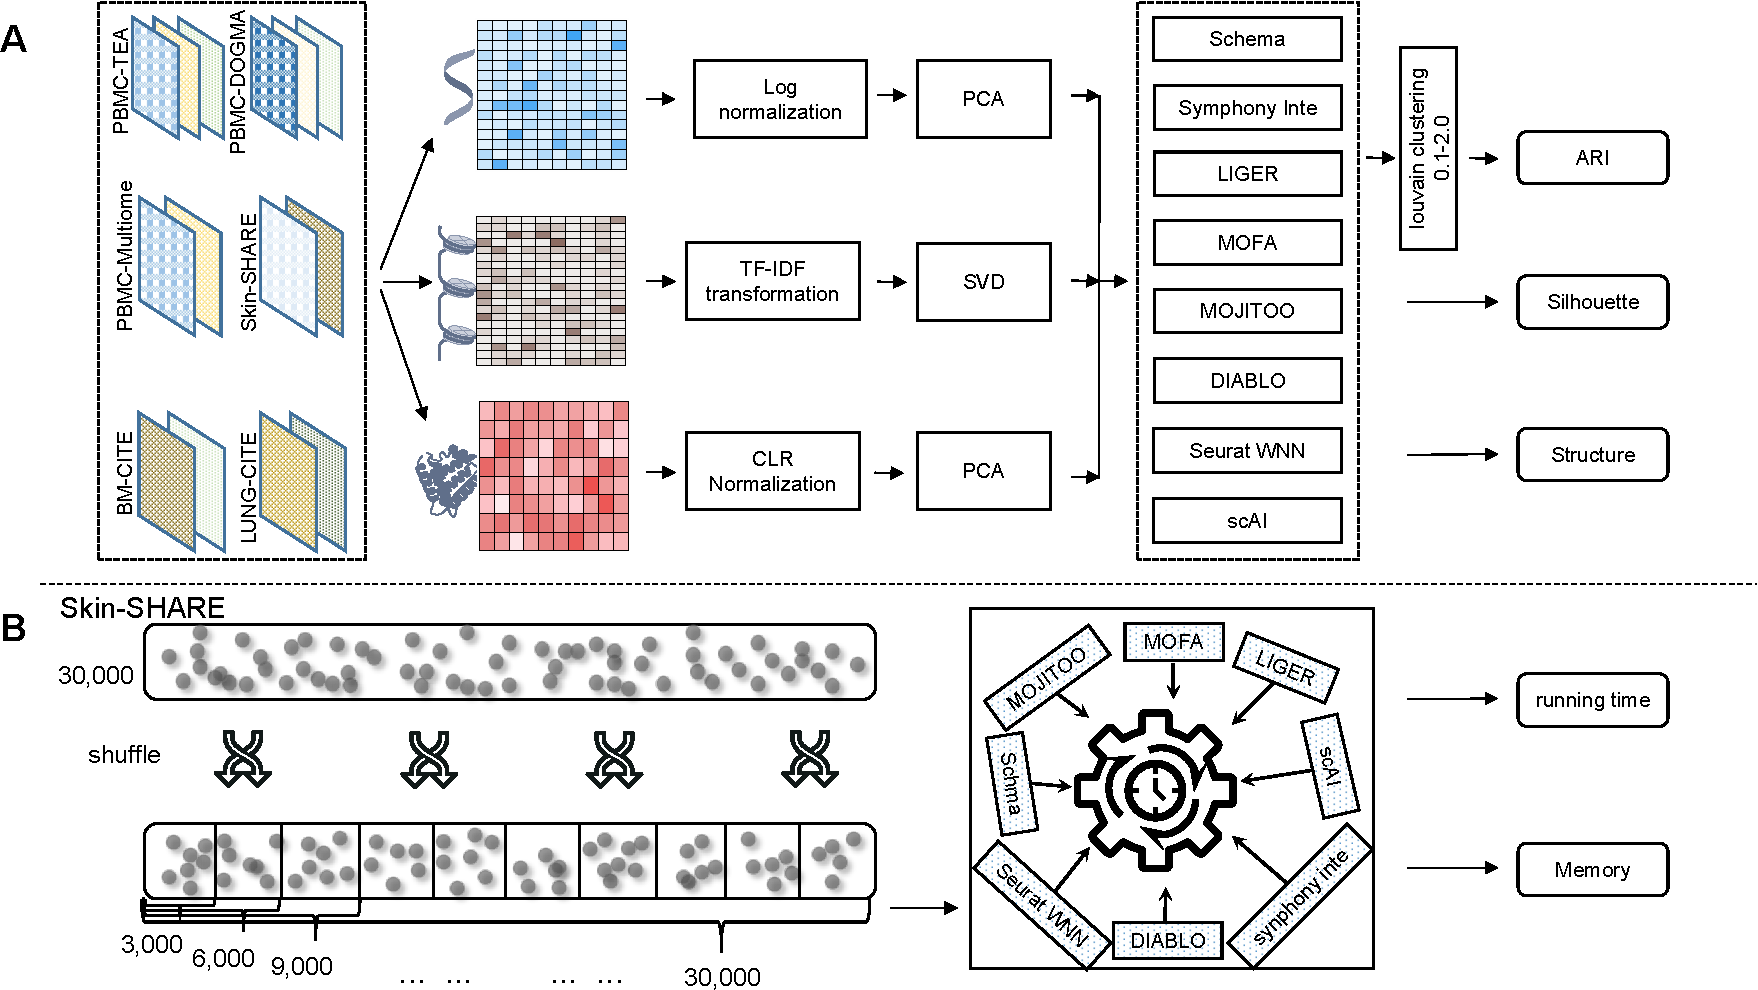
\includegraphics[width=0.95\textwidth]{evaluation_MOJITOO/fig}
	\vspace{0.1cm}
	\caption[evaluation\_MOJITOO]{
	evaluation\_MOJITOO.}
	\label{fig:evaluation_MOJITOO}
\end{figure}

\subsection{integration}
\begin{description} %%formula
	\item[Requirements of Memory and Running Time].
	\item[Space Presevation]. 
	\item[Distance Accuracy]. 
  silhouette to latent space to evaluate the performance of these methods. For each data point $i\in C_i$, where $C_i$ is the label of the data point, we calculate the inner cluster mean distance:
\begin{equation}
  a(i) = \frac{1}{|C_i| - 1} \underset{j \in c_i, i\neq j}{\sum} d(i, j)
\end{equation}
Next, the smallest mean out cluster distance to data point $i$ is:
\begin{equation}
b(i) = \underset{k\neq i}{\min}\frac{1}{|C_k|}\underset{j\in c_k}{\sum} d(i,j)
\end{equation}
The solhoutte index is defined as:
\begin{equation}
s(i)=\frac{b(i)-a(i)}{\max\{a(i), b(i)\}}, -1\leq s(i) \leq 1
\end{equation}
where $d(i,j)$ is the distance of two cells under some specific latent space, here we considered both euclidean distance and cosine distance.

	\item[clustering Accuracy]. 
\end{description}
% to validate improve the perfomance, ---> PBMC capture major cell types and subtype changings
\subsection{Downstream Analysis methods}

% Nemenyi post-hoc test
\subsection{???Statistical Methods}



\subsection{Execution of trajectory inference}
% List how to install and run the competing methods
% how to set up dynverse environment
\subsubsection{competing methods}
\begin{description}
	\item[slingshot] We installed ..... to perform	
\end{description}

\subsection{Evaluation of trajectory inference}
% dynverse benchmarking selected metrics description
\begin{figure}[!ht]
	\centering
	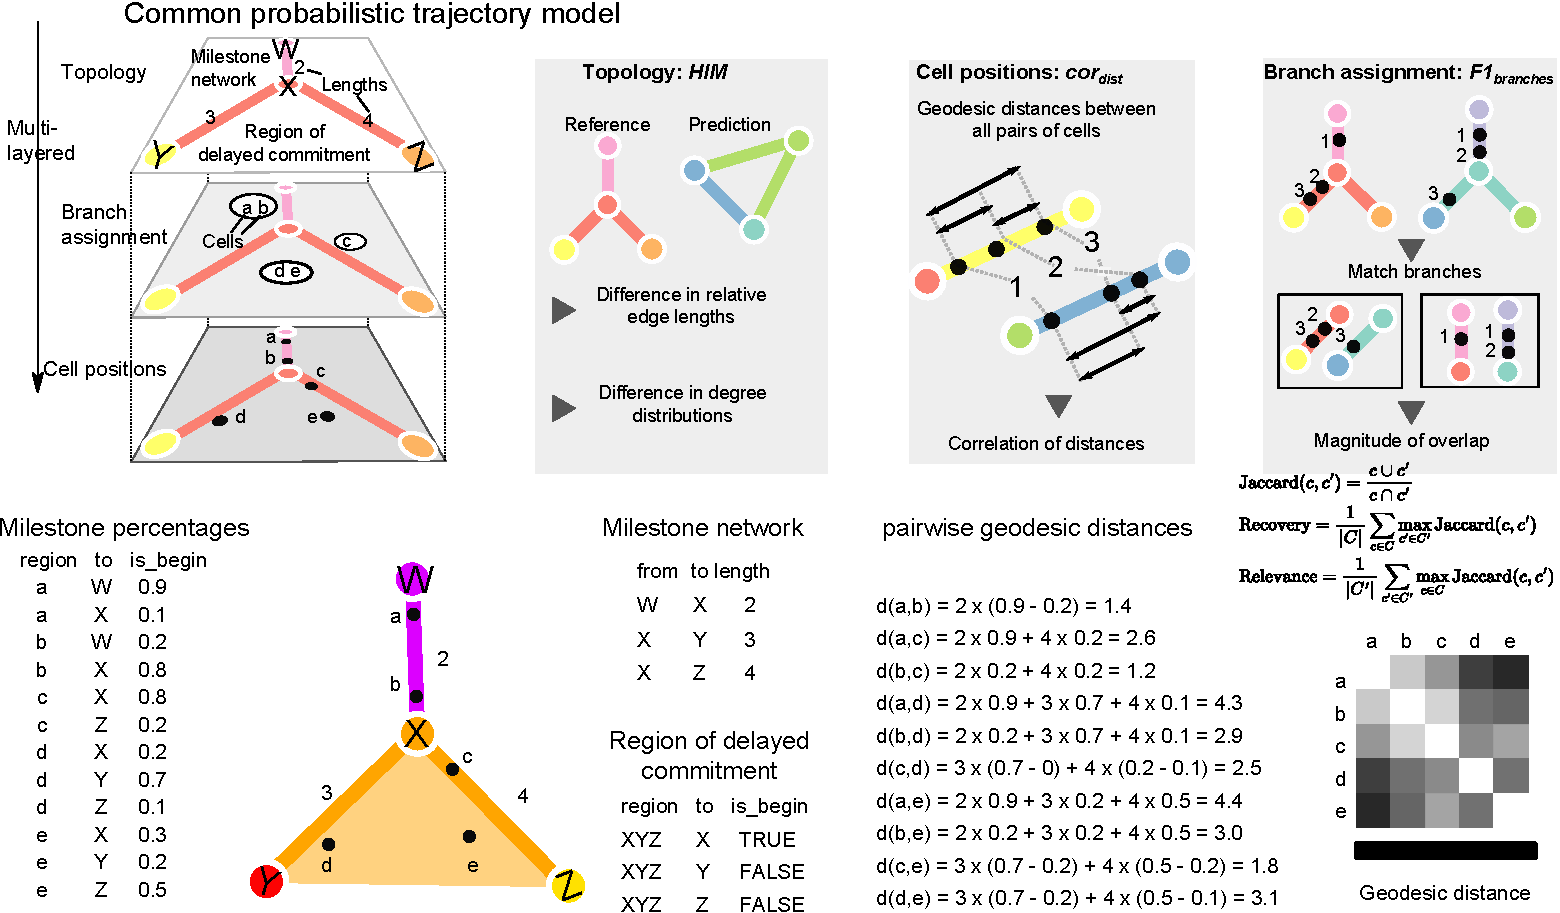
\includegraphics[width=0.95\textwidth]{dynverse_metrics/fig}
	\vspace{0.1cm}
	\caption[dynverse\_metrics]{
	dynverse\_metrics.}
	\label{fig:dynverse_metrics}
\end{figure}

\begin{figure}[!ht]
	\centering
	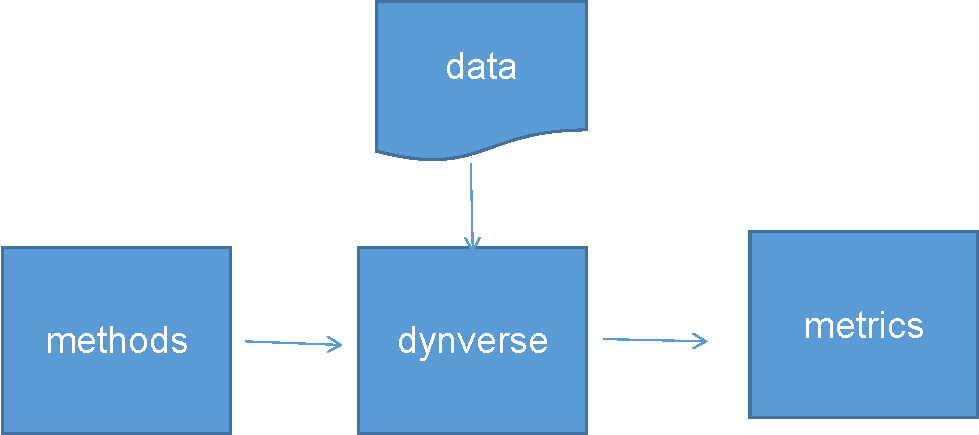
\includegraphics[width=0.95\textwidth]{evaluation_PHLOWER/fig}
	\vspace{0.1cm}
	\caption[evaluation\_PHLOWER]{
	evaluation\_PHLOWER.}
	\label{fig:evaluation_PHLOWER}
\end{figure}



\section{Biological Validatation}
\subsection{Apply integration \& trajectory inference to kidney organoid data}
\subsection{Characterize the cell fate xxxx}

\section{Discussion}

